\chapter{Path Planning}

\textbf{Path Planning} is a geometric problem, related to finding a path from a starting point to a goal point while satisfying a set of constraints, such as: restricting the solutions inside the robot's configuration space, avoiding obstacles in the task space, avoiding singularity points and respecting the robot's 
joint limits.
%
\section{Path planning sampling methods}
%
Sampling planning methods use random functions to choose a sample from the configuration or joint space. Unlike discretizing methods, sampling ones are 
computationally inexpensive cannot compute optimal solutions.
%
\subsection{RRT Algorithm}
%
The \textbf{Rapidly-exploring Random Trees} algorithm searches for an obstacle-free motion plan from an initial state $x_{init}$ to a set of goal states $\mathcal{X}_{goal}$ that are within the allowed position and orientation tolerances.

\small
\begin{algorithm}[H]
\SetAlgoLined
\ForEach{replanning attempt}{
	initialize vertices $V \leftarrow \lbrace x_{init} \rbrace$\;
	initialize edges $E \leftarrow \varnothing$\;
	initialize search tree $T \leftarrow (V,E)$\;
	\While{$time \leq maxPlanningTime$}{
		$x_{rand} \leftarrow$ getSampleStateFrom($\mathcal{X}$)\;
		$x_{nearest} \leftarrow$ getNearestNodeInTreeToState($T, x_{rand}$)\;
		$x_{new} \leftarrow$ findLocalPlanFromTo($x_{nearest}, x_{rand}$)\;
		\If{isPathCollisionFree($x_{nearest}, x_{rand}$)}{
			$V \leftarrow V \cup \lbrace x_{new} \rbrace $\;
			$E \leftarrow E \cup \lbrace (x_{nearest}, x_{rand}) \rbrace $\;
			\If{$x_{new} \in \mathcal{X}_{goal}$}{
				\Return SUCCESS and path plan $ T=(V,E) $ \;
			}
		}
	}
}
\Return FAILURE and $ T=(V,E) $ \;
\caption{RRT Algorithm}
\end{algorithm}
\nprmalsize

Other variations of the RRT Algorithm, which are also available in the OMPL library, included in the MoveIt library of ROS framework  are:
a) \textbf{TRRT} Transition-based RRT, b) \textbf{BiTRRT} Bidirectional Transition-based RRT, c) \textbf{RRT*}
	\item \textbf{RRTConnect} with is the default OMPL path planner in ROS, d) \textbf{LBTRRT} Lower Bound Tree RRT.
%
\subsection{PRM Algorithms}
%
The \textbf{Probabilistic Roadmap} (PRM) algorithm constructs a roadmap representation of $\mathcal{C}_{free}$ \textbf{before searching} for a solution. After the roadmap is successfully built, then the algorithm searches for a solution using a traditional graph-based search algorithm. The sampling of the free configuration space is usually performed using a uniform distribution except from the regions close to objects where the sampling is more dense.

\begin{algorithm}[H]
\SetAlgoLined
initialize vertices $V \leftarrow \lbrace x_{init} \rbrace$\;
initialize edges $E \leftarrow \varnothing$\;
initialize roadmap graph $G \leftarrow (V,E)$\;
\For{$i = 1, \ldots , n$}{
	$x_{rand,i} \leftarrow$ getSampleStateFrom($\mathcal{X}$)\;
	$\mathcal{N}(x_{rand,i}) \leftarrow$ getKNearestNeighbors($G=(V,E), x_{rand,i}$)\;
	$V \leftarrow V \cup \lbrace x_{rand,i} \rbrace $\;
	\ForEach{$x \in \mathcal{N}(x_{rand,i})$}{
		\If{there is no edge between $x$ and $x_{rand,i}$}{
			\If{isPathCollisionFree($x_{nearest}, x_{rand,i}$)}{
				$E \leftarrow E \cup \lbrace (x_{rand,i}, x), (x, x_{rand,i}) \rbrace$
			}
		}
	}
}
\Return $G=(V,E)$
\caption{PRM roadmap construction (preprocessing phase)}
\end{algorithm}

Other variations of the PRM Algorithm, which are also available in the OMPL library, included in the MoveIt library of ROS framework  are: i) \textbf{PRM*}, ii)  \textbf{LazyPRM}, and iii) \textbf{LazyPRM*},
%
\section{Pick and place algorithm}
%
% Help on using the algorithme package
% http://ftp.ntua.gr/mirror/ctan/macros/latex/contrib/algorithm2e/doc/algorithm2e.pdf 
\begin{algorithm}[H]
\SetAlgoLined
\ForEach{surgical tool}{
	\tcc{Plan the Pick pipeline}
	set grasp pose\;
	set pre-grasp approach\;
	set post-grasp retreat\;
	set posture of eef before grasp (open gripper)\;
	set posture of eef during grasp (closed gripper)\;
	\tcc{Plan the Place pipeline}
	set place location pose\;
	set pre-place approach\;
	set post-grasp retreat\;
	set posture of eef after placing object\;
	Plan pick and place paths\;
}
\caption{Pick and Place algorithm}
\end{algorithm}

Picking and placing small objects results in a straightforward path planning. When the object to be picked has at least one dimension significantly larger than the others, like a rod such similar to the surgical tools,  then the path planning becomes more complicated, because of the possible  collisions of the tool with the links of the rest of the robot (the link of the end-effector will probably not collide with the tool).
%
\section{Task space analysis}
%
%Before designing any paths and trajectories it is very important to better understand the taskspace in which the surgical tool will operate in. 
When the robot arm is in the pick-and-place phase where it detects the surgical tool and grasps and then move to the mounting dock to insert it, then at this phase, the taskspace is the same as the robot's taskspace. However, when the surgical tool is inserted in the patient's body and starts executing pivoting motions, then there are two taskspaces tto be studied. The first one is the surgical taskspace, which is where the surgical movements are planned (sutures, laparoscopic camera movements etc.) and the second taskspace is the one outside of patient's body in which the planned paths are "mirrored" so that the robot can execute them. The surgical taskspace $\mathbb{S}$ is the one shown in Figure~\ref{surgical-taskspace}. The paths inside the surgical task are transformed via the Fulcrum effect transformation, described in more detail in Section~\ref{section:fulcrum-effect}, to the pivot paths taskspace $\mathbb{P}$ which is a subset of the robot's taskspace $\mathbb{T}$ (we assume that all pivot motions can be executed, i.e. that all motions are reachable and fully inside the robot's taskspace). The paths are then used as input to a trajectory generator whose output 
is transformed via the IK equations to the joint angles that belong to the joint space $\mathbb{J}$. 

Alternatively in a mathematical notation, the fulcrum effect transformation is $
Φ: \mathbb{S} \longrightarrow \mathbb{P}
$, while the IK transformation is $
IK: \mathbb{P} \subset \mathbb{T} \longrightarrow \mathbb{J}
$
and similarly the forward kinematics transformation can be described as $
FK: \mathbb{J} \longrightarrow \mathbb{T}
$\\
%
\begin{center}
\begin{figure}[!htb]
\centering

\includegraphics[width=0.7\textwidth]{images/spaces-and-transformations.png}\\
\caption{Relationships beteeen Surgical and pivot path taskspace.}
\label{surgical-taskspace}
\end{figure}
\end{center}

The Dexterity metric of the tool's task space is
\begin{eqnarray}
\mathcal{D} &=& \mathcal{L}_q \mathcal{M}, \mbox{where}
\label{dexterity-measure}
\\
\mathcal{M} &=& \sqrt{det(J J^\top)}\\
\label{joint-limit-measure}
\mathcal{L}_{q}&=&1-\exp\left\{-\kappa\prod_{i=1}^{n_{k}}\frac{(q_{ {i}}-q_{i,\min})(q_{i,\max}-q_{i})}{(q_{i,\max}-q_{i,\min})^{2}}\right\}
\end{eqnarray}

\begin{center}
\begin{figure}[htbp]
\centering
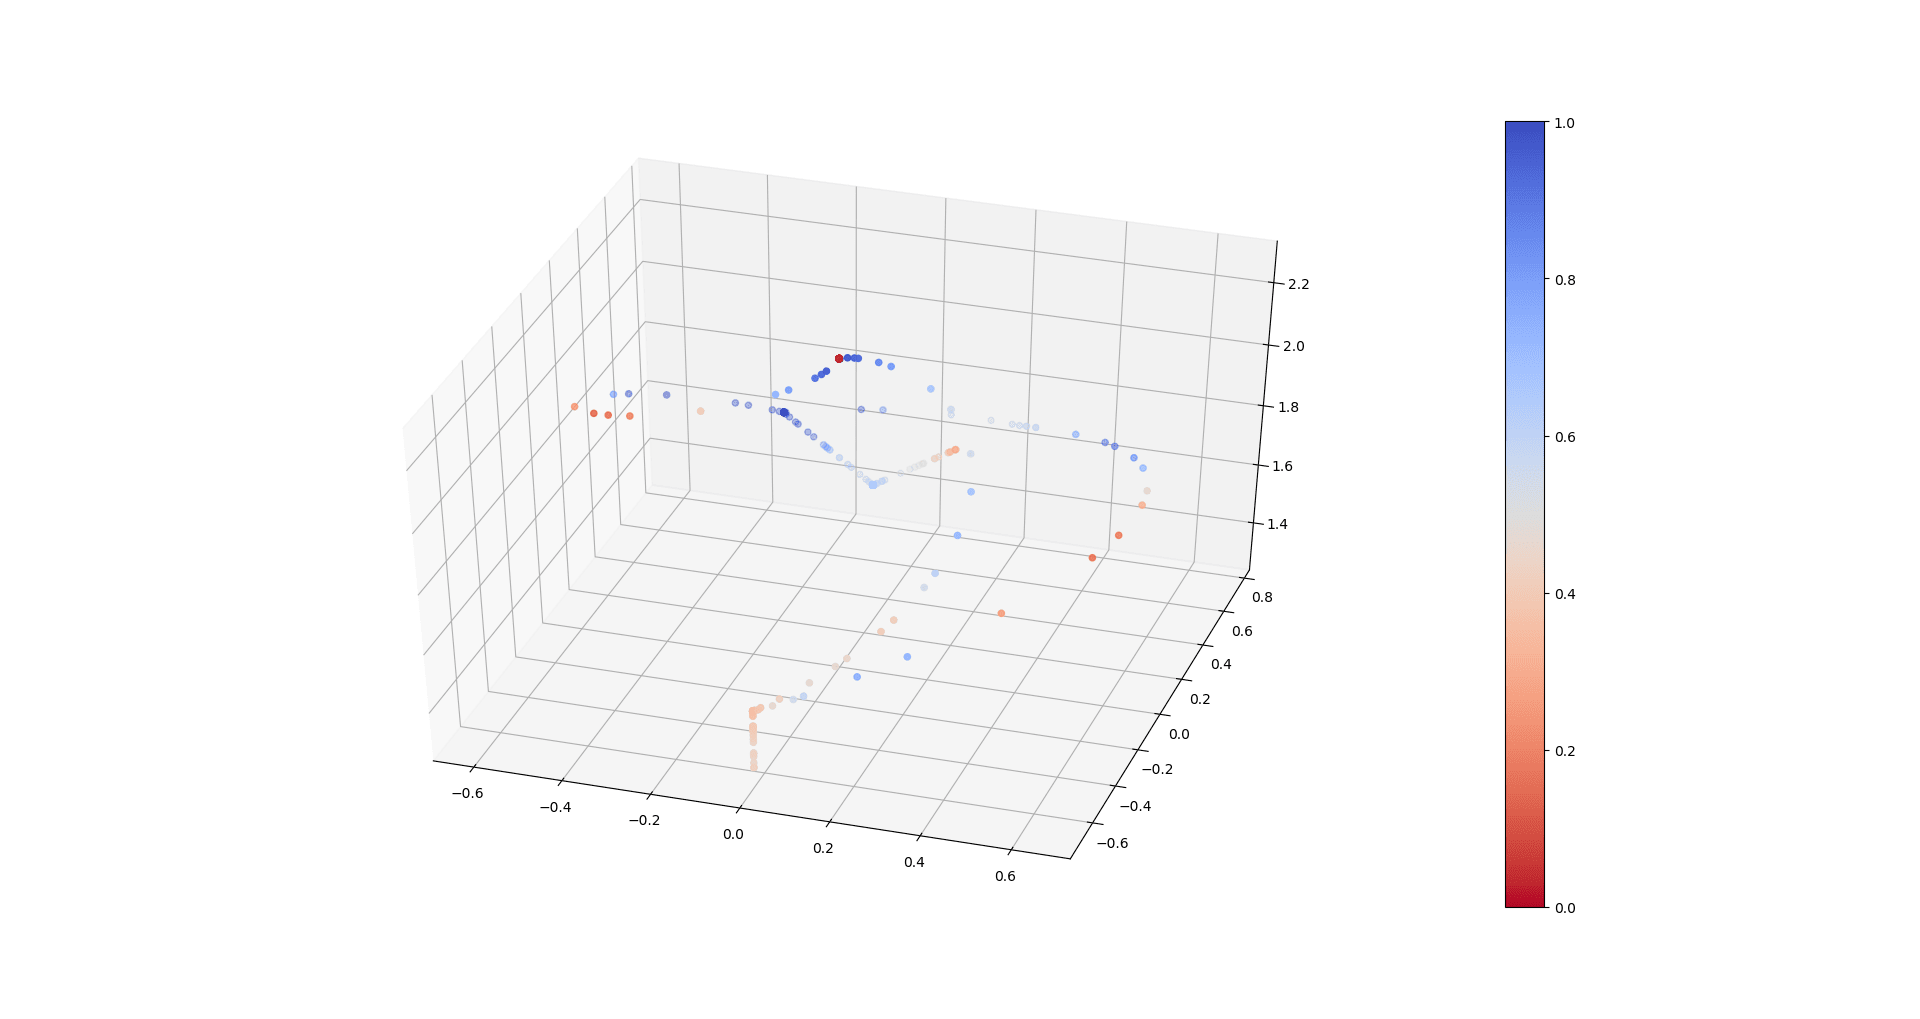
\includegraphics[width=0.7\textwidth]{images/robot-planner1-manipulability-plot.png}\\
\caption{Manipulability index of robot arm during  trajectory}
\label{robot-planner1-manipulability-plot}
\end{figure}
\end{center}

Equation~(\ref{joint-limit-measure}) calculates a joint limit measure which is multiplied with the manipulability measure and gives the dexterity measure and the following:
a) If $q_i = q_{min}$ or $q_i = q_{max}$ then the exponential is equal to 1 which means that $\mathcal{L}_{q}$ and $\mathcal{D}$ are both 0, implying that the robot has \textbf{no dexterity at the boundary of the task space}, b) If the value of $q_i$ is close to its boundary value then the dexterity approaches zero. The distance from the boundary (or in other words how fast the exponential term converges) depends on the parameter $\kappa$, and c) The $q_{min}, q_{max}$ are calculated from the geometry of the task-space.

For maximum dexterity throughout the trajectory in a pivoting motion, the pivot sub-taskspace (i.e. the space of all configurations of feasible pivot motions) must be fully within the robot’s whole reachable taskspace, otherwise only a small range of pivot movements will be 
feasible. 
Finding $q_{i,min}, q_{i,max}$ at (\ref{joint-limit-measure}) is difficult and time-consuming at task spaces with more intricate geometries. A similar and more practical equation to (\ref{joint-limit-measure}) can be written for calculating the dexterity of the robot in task space:
\begin{equation}
\label{rcm-taskspace-limit-measure}
\mathcal{L}_{p}=1-e^{-\kappa (r_{max} - r)},
\end{equation}
where $r_{max}$ is the maximum radius of a circle that the tool tip can follow at a given insertion depth $z$. Moreover, at every point of the taskspace, $L^2 = r^2 + z^2$. Equation (\ref{rcm-taskspace-limit-measure}) shows dexterity in terms of approaching the boundary of the taskspace and it does not take into consideration internal points of low dexterity and singularities like (\ref{dexterity-measure}).

\begin{listing}[H]
\begin{minted}[tabsize=2,breaklines,frame=lines,framesep=2mm,baselinestretch=1.2,fontsize=\footnotesize, linenos]{matlab}
x = []; y = []; z = []; r = [];
s = 0:0.005:0.5; L = 0.48; k = 4.5;
for z0=-L:0.01:0
    if abs(z0)*sqrt(2) <= L
        rmax = abs(z0);
    else
        rmax = sqrt(L^2-z0^2);
    end
    for r0=0:0.02:rmax
        x = [x, r0*\cos(2*pi*s)];
        y = [y, r0*\sin(2*pi*s)];
        z = [z, z0*ones(size(s))];
        lp = 1-exp(-k*(rmax-r0));
        r = [r, lp*ones(size(s))];
    end
end
\end{minted}
\caption{RCM Taskpace calculation in MATLAB}
\label{code:rcm_taskspace_matlab}
\end{listing}

\begin{center}
\begin{figure}[htbp]
\centering
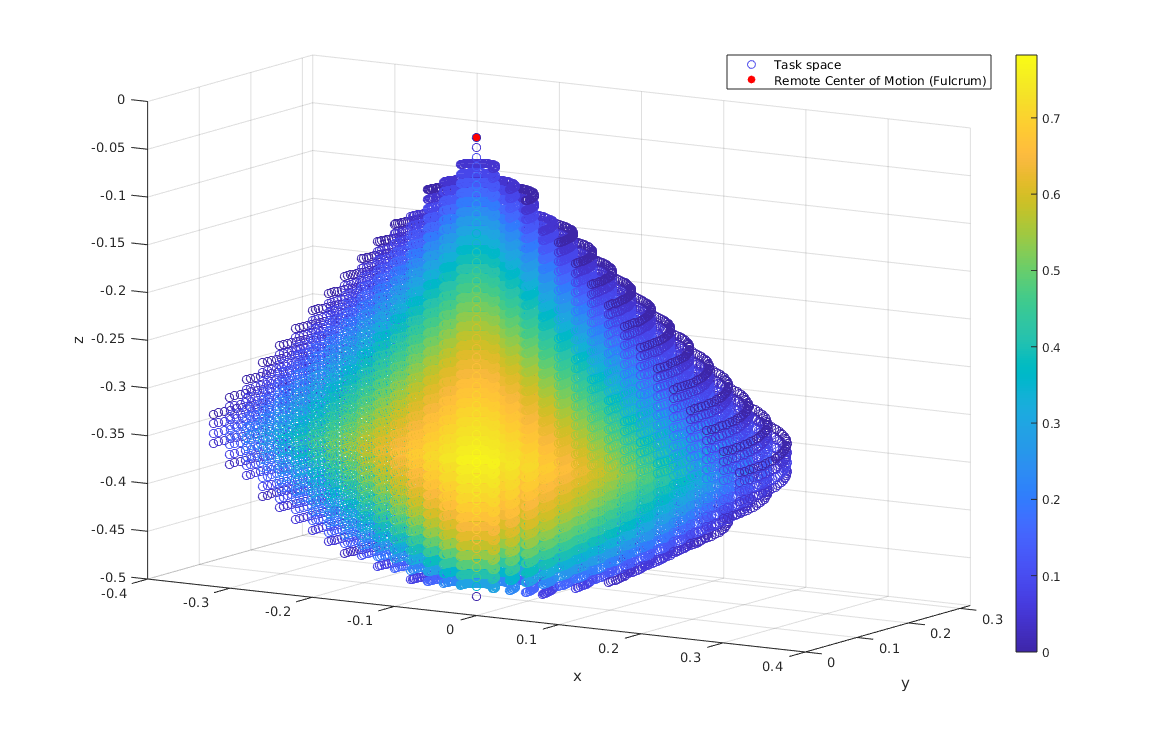
\includegraphics[width=0.7\textwidth]{images/rcm_taskspace.png}\\
\caption{Task space inside patient's body. Colors with 0 or low value correspond to points with low dexterity.}
\label{surgical-taskspace}
\end{figure}
\end{center}

All of the metrics above, measure how much reachable are various points of the surgical taskspace, but they are calculated from different perspectives, using input values from different spaces.
\begin{equation}
\mathcal{L}_{q}, \mathcal{M}: \mathbb{J} \longrightarrow \mathbb{R} \quad \textrm{and} \quad
\mathcal{L}_{p}: \mathbb{S} \longrightarrow \mathbb{R}
\end{equation}